\documentclass[11pt]{article}
\usepackage[letterpaper,margin=0.6in]{geometry}
\usepackage{booktabs,graphicx,amsmath,amssymb}
\setlength{\parindent}{0pt}
\setlength{\parskip}{5pt}
\pagestyle{plain}
\begin{document}
\begin{center}\large\textbf{Section 6.3: Individual Rationality and Collective Outcomes}\\[4pt]
\normalsize Revised figure sequence and appendix placement\end{center}
\begin{enumerate}
\setlength{\itemsep}{10pt}
\item \textbf{Bar and CDF panels (Figure 1).} Show group CCEI and CEIV by members' individual CCEI
categories, using the pooled median across both waves (0.9806594). High means strictly above this median
and Low otherwise. The CDF panels complement the mean comparisons
by showing the full distributions, including the mass at one.

\item \textbf{Four joint outcomes (Figure 2).} Place group CCEI status on the horizontal axis and group CEIV
status on the vertical axis. Each quadrant reports its count and share of the 1,304 pair-wave observations:
both below one: 415 (31.8\%); only CCEI equal to one: 117 (9.0\%); only CEIV equal to one: 300 (23.0\%); both equal to one: 472 (36.2\%). These are categorical quadrants, with each index either below one or equal to one.

\item \textbf{Average marginal effects (Figure 3).} Use the pooled four-outcome multinomial logit with both
members' individual CCEIs, student, friendship, and choice-pattern controls, and class fixed effects.
For a 0.1 increase in maximum individual CCEI, the average marginal effect on the probability of both group
indices equaling one is +19.2 percentage points; the corresponding minimum-CCEI effect is +2.4 percentage
points. Both are positive with 95\% confidence intervals excluding zero. Minimum individual CCEI also has
a positive effect on the CCEI$=1$, CEIV$<1$ outcome. These estimates describe conditional associations;
the plot does not test equality of the two members' effects.
\end{enumerate}

\textbf{Appendix Table A1.} Retain only columns (1)--(3) of the attached table, with both group CCEI and CEIV
panels. Column (1) includes class fixed effects; column (2) adds student, friendship, and choice-pattern controls;
column (3) uses these controls with pair fixed effects. Low--Low is the omitted category.
Group CCEI: High--High minus Low--High comparison $p$-values are $<0.001$, $<0.001$, 0.045 in columns (1)--(3), respectively.
Group CEIV: High--High minus Low--High comparison $p$-values are 0.111, 0.168, 0.991 in columns (1)--(3), respectively.

\textit{Measurement and sample:} CEIV is used throughout. All figures and appendix regressions use
1,304 pair-waves from 652 pairs in 64 classes. CEIV$=1$ denotes rationalizability under the specified
individual calibrations and varying weights; it does not identify actual aggregation weights or a communication
process. Figure and table numbers in this review packet indicate the proposed sequence within Section 6.3.

\clearpage
\begin{center}\large\textbf{Figure 1: Collective CCEI and CEIV}\\
\normalsize By members' individual CCEI category\end{center}
\begin{center}
\begin{minipage}{0.485\textwidth}\centering
\includegraphics[width=\linewidth]{group_ccei_bar.pdf}\\[-2pt]
(a) Mean collective CCEI
\end{minipage}\hfill
\begin{minipage}{0.485\textwidth}\centering
\includegraphics[width=\linewidth]{group_ccei_cdf.pdf}\\[-2pt]
(b) CDFs of collective CCEI
\end{minipage}

\vspace{3pt}
\begin{minipage}{0.485\textwidth}\centering
\includegraphics[width=\linewidth]{group_ceiv_bar.pdf}\\[-2pt]
(c) Mean collective CEIV
\end{minipage}\hfill
\begin{minipage}{0.485\textwidth}\centering
\includegraphics[width=\linewidth]{group_ceiv_cdf.pdf}\\[-2pt]
(d) CDFs of collective CEIV
\end{minipage}
\end{center}
\footnotesize
\textit{Notes:} Each member is High if individual CCEI exceeds the pooled median across both waves
(0.9806594), and Low otherwise; no individual CCEI equals the median. The sample contains 1,304 pair-waves
from 652 pairs. Low--Low, Low--High, and High--High contain
348, 608, 348 pair-waves, respectively.
Bars show unadjusted means with 95\% Student-$t$ confidence intervals. Bracket labels are upper-category
minus lower-category means; significance uses Welch two-sample $t$-tests. CDFs use all observations,
including the mass at one. These descriptive intervals and tests do not adjust for class clustering;
Figure 3 and Appendix Table A1 do. +, *, and ** denote $p<0.10$, $p<0.05$, and $p<0.01$.

\clearpage
\normalsize
\begin{center}\large\textbf{Figure 2: Joint Collective Outcomes}\\
\normalsize Counts and shares by group CCEI and CEIV status\end{center}
\begin{center}
\includegraphics[width=0.95\textwidth]{joint_outcome_quadrants.pdf}
\end{center}
\footnotesize
\textit{Notes:} The horizontal axis classifies group CCEI and the vertical axis classifies group CEIV.
Diagonal cells are blue and off-diagonal cells are white; stripes and dots distinguish outcomes within each color.
Each quadrant reports the observed count and percentage of all 1,304 pair-waves from 652 pairs in 64 classes;
each pair contributes one observation in each of two waves. These are pooled pair-wave frequencies,
rather than a classification of unique pairs. Percentages sum to 100\% before rounding.
An index is classified as one at values at least $1-10^{-9}$; all other observations are below one.
CEIV endpoint classifications agree with both supplied numerical bounds. The axes represent binary status,
rather than distances between continuous index values. CEIV$=1$ denotes rationalizability under the specified
individual calibrations and varying weights.

\clearpage
\normalsize
\begin{center}\large\textbf{Figure 3: Individual Rationality and Joint Collective Outcomes}\end{center}
\begin{center}
\begin{minipage}{0.82\textwidth}\centering
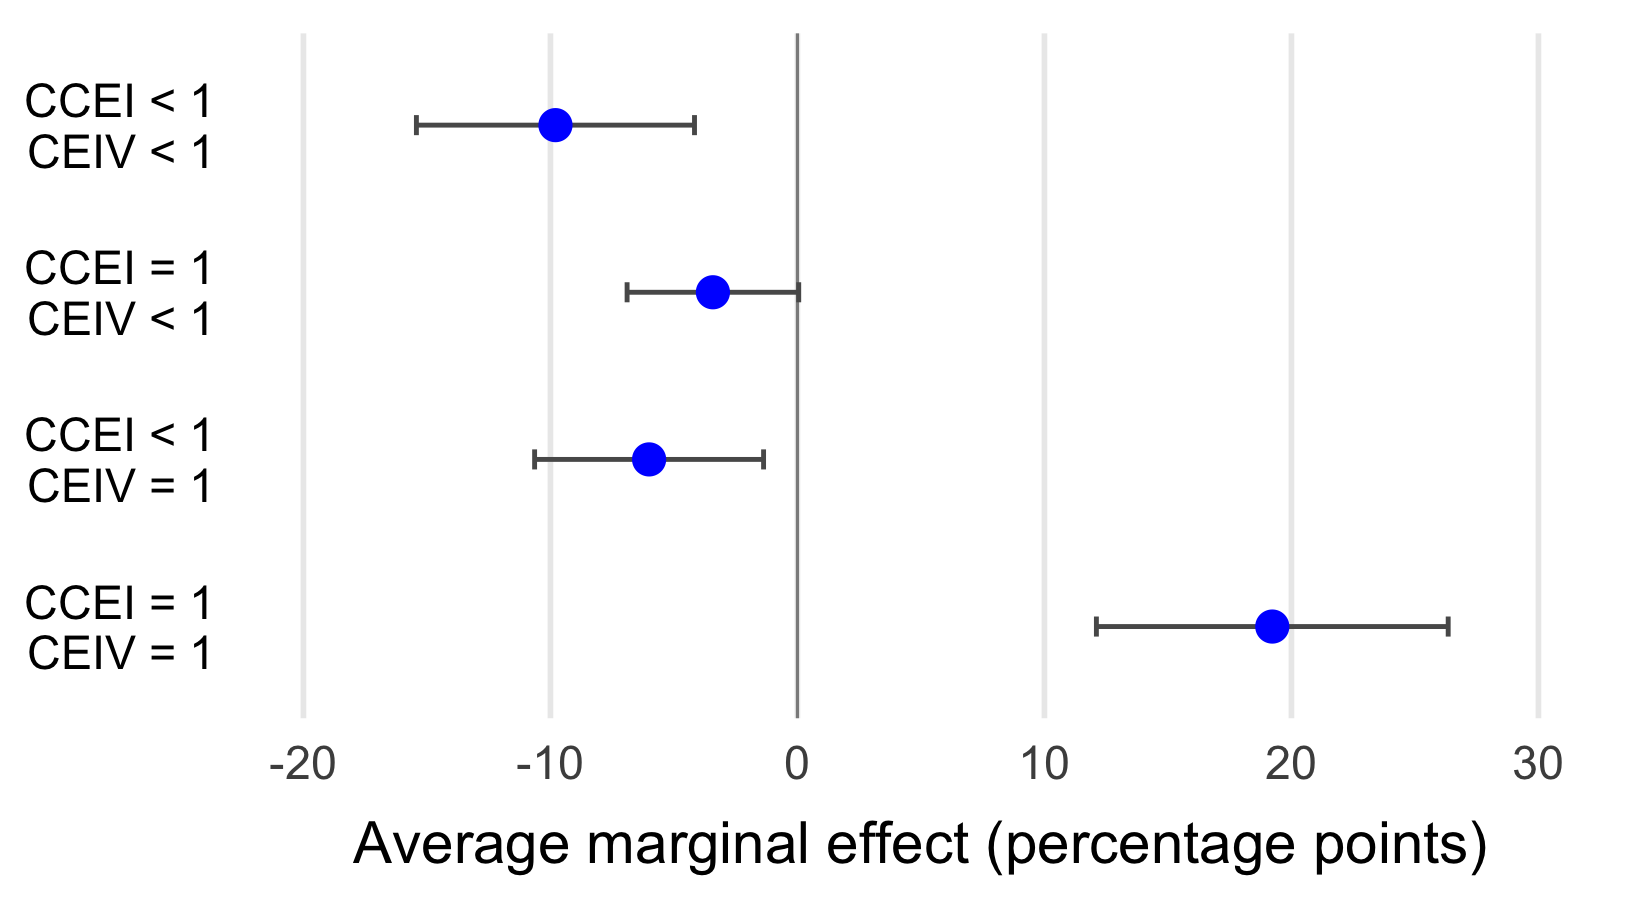
\includegraphics[width=\linewidth]{figure6_a_ame_maximum.png}\\
(a) $\mathrm{CCEI}_{\max,gt}$
\end{minipage}

\vspace{4pt}
\begin{minipage}{0.82\textwidth}\centering
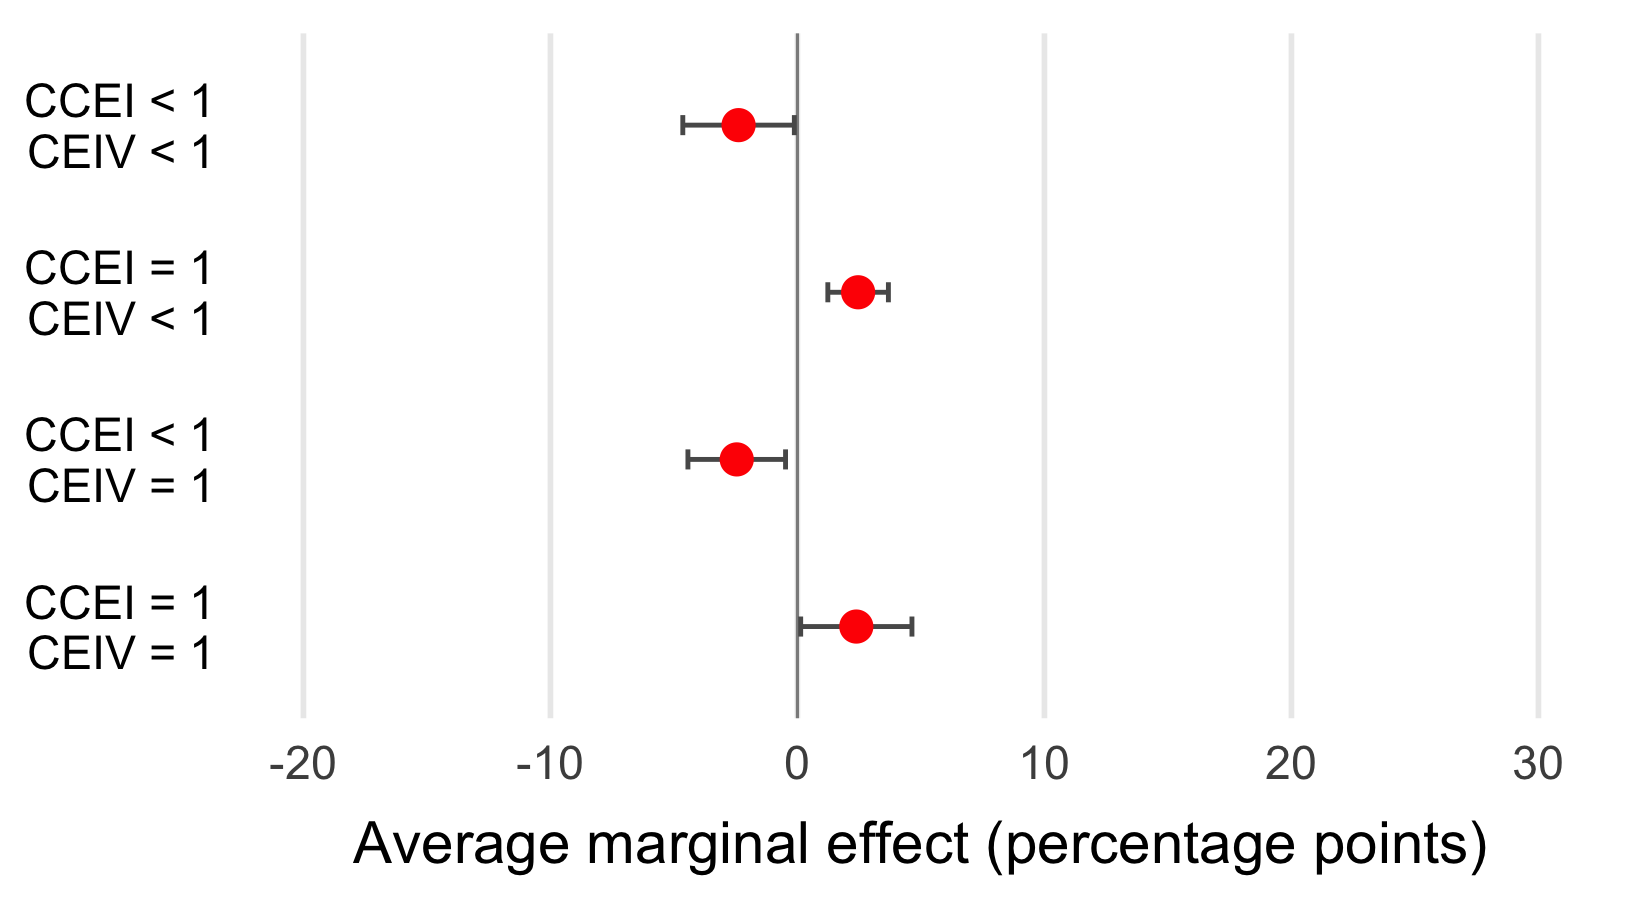
\includegraphics[width=\linewidth]{figure6_a_ame_minimum.png}\\
(b) $\mathrm{CCEI}_{\min,gt}$
\end{minipage}
\end{center}
\footnotesize
\textit{Notes:} Pooled four-category multinomial-logit average marginal effects, expressed in percentage points
and scaled to a 0.1 increase in the indicated member's individual CCEI. These are scaled average derivatives,
rather than exact finite changes in predicted probabilities. Both individual CCEIs enter jointly, with student,
friendship, and corner/midpoint share controls and class fixed effects. The control set matches Appendix
Table A1, Column (2); risk-aversion controls and wave fixed effects are excluded.
The sample is 1,304 pair-waves from 652 pairs in 64 classes. Horizontal bars are 95\% normal confidence intervals
based on class-clustered standard errors. Effects sum to zero across the four outcomes for each member.
An index is classified as one within a numerical tolerance of $10^{-9}$. The joint-outcome counts and shares
appear in Figure 2. CEIV$=1$ denotes rationalizability under the specified individual calibrations and varying
weights; it does not identify actual aggregation weights or a communication process.
The effects describe conditional associations.

\clearpage
\normalsize
\setlength{\parskip}{3pt}
\begin{center}\large\textbf{Appendix Table A1: Individual Rationality and Collective Outcomes}\\
\normalsize Columns (1)--(3) of the attached table\end{center}
\begin{center}\small
\setlength{\tabcolsep}{14pt}
\renewcommand{\arraystretch}{1.12}

\begin{tabular}{lccc}
\toprule
& \multicolumn{3}{c}{Individual CCEI category dummies}\\
\cmidrule(lr){2-4}
& (1) & (2) & (3)\\
\midrule
\multicolumn{4}{l}{\textit{Panel A: Group CCEI}}\\[3pt]
Low--High pair & 0.044\textsuperscript{**} & 0.043\textsuperscript{**} & 0.036\textsuperscript{**}\\
 & (0.011) & (0.011) & (0.013)\\
High--High pair & 0.078\textsuperscript{**} & 0.075\textsuperscript{**} & 0.054\textsuperscript{**}\\
 & (0.010) & (0.010) & (0.013)\\
\midrule\multicolumn{4}{l}{\textit{Post-estimation comparisons}}\\[2pt]
High--High minus Low--High & 0.034 & 0.031 & 0.018\\
Standard error of difference & 0.008 & 0.007 & 0.009\\
$p$: High--High = Low--High & $<0.001$ & $<0.001$ & 0.045\\
\addlinespace
Observations & 1,304 & 1,304 & 1,304\\
$R^2$ & 0.130 & 0.159 & 0.631\\
\midrule
\multicolumn{4}{l}{\textit{Panel B: Group CEIV}}\\[3pt]
Low--High pair & 0.039\textsuperscript{**} & 0.040\textsuperscript{**} & 0.033\textsuperscript{**}\\
 & (0.010) & (0.010) & (0.011)\\
High--High pair & 0.051\textsuperscript{**} & 0.050\textsuperscript{**} & 0.033\textsuperscript{*}\\
 & (0.010) & (0.010) & (0.013)\\
\midrule\multicolumn{4}{l}{\textit{Post-estimation comparisons}}\\[2pt]
High--High minus Low--High & 0.012 & 0.010 & 0.000\\
Standard error of difference & 0.007 & 0.007 & 0.010\\
$p$: High--High = Low--High & 0.111 & 0.168 & 0.991\\
\addlinespace
Observations & 1,304 & 1,304 & 1,304\\
$R^2$ & 0.096 & 0.114 & 0.589\\
\midrule
Fixed effects & Class & Class & Pair\\
Student and friendship controls &  & $\checkmark$ & $\checkmark$\\
Corner/midpoint share controls &  & $\checkmark$ & $\checkmark$\\
\bottomrule
\end{tabular}
\end{center}
\footnotesize
\textit{Notes:} OLS regression coefficients have class-clustered standard errors in parentheses. All columns
use 1,304 pair-waves from 652 pairs in 64 classes. Low--Low is omitted. High means individual CCEI exceeds
the pooled median across both waves (0.9806594), and Low otherwise, as in Figure 1. Column (1) includes
class fixed effects; Column (2) adds full controls with class fixed effects; Column (3) uses full controls
with pair fixed effects.

The post-estimation section reports the linear contrast $\beta_{HH}-\beta_{LH}$ and its class-clustered
standard error; the contrast is not an additional regressor. Its two-sided $p$-value tests
$H_0:\beta_{HH}=\beta_{LH}$ using the estimated coefficient covariance.

Full controls comprise pair maxima and absolute differences in math score, height, Big Five traits,
network degree, popularity, and exact corner/equal-allocation shares, with mixed-gender, friendship,
and missing-value indicators. Risk-aversion controls and wave fixed effects are excluded.
Estimates and category comparisons describe conditional associations. +, *, and ** denote significance
at the 10\%, 5\%, and 1\% levels.
\end{document}
